\mode*

\section{Disposition}

\begin{frame}
  \begin{figure}
    
\includegraphics[height=0.8\textheight]{fig/book.jpg}
    \caption{Front cover of Necessary Conditions of Learning.}
  \end{figure}
\end{frame}

\begin{frame}
  \begin{enumerate}
    \item What makes humans human?
    \item What is to be learned?
    \alert{\item Sameness and difference in learning}
    \item What does the world look like to others?
    \item The art of learning
    \item Making learning possible
    \item Learning to help others to learn
  \end{enumerate}
\end{frame}

\begin{frame}
  \begin{block}{Ch 3 Sameness and difference in learning}
    \begin{itemize}
      \item The problem with direct reference (induction).
      \item The patterns: contrast, generalization, fusion.
      \item \textcquote[p.~71]{NecessaryConditionsOfLearning}{%
          \textins{P}racticing something other than what was tested was more 
          effective than practicing exactly what was tested.%
        }
    \end{itemize}
  \end{block}
\end{frame}

\begin{frame}
  \begin{example}[Physics]
    \begin{enumerate}
      \item Students were introduced to modern physics.
      \item Students were introduced to modern physics, contrasted with what we 
        believed before.
    \end{enumerate}
  \end{example}
\end{frame}

\begin{frame}
  \begin{example}[Using the known to prepare for unknown]
    \begin{itemize}
      \item Kids were to hit a target by throwing a shuttlecock (badminton 
        \enquote{ball}).
    \end{itemize}
    \begin{enumerate}
      \item Practicing from the same position as testing.
      \item Practicing from several positions, except the testing position.
    \end{enumerate}
  \end{example}
\end{frame}

\section{An experiment}

\begin{frame}
  \begin{center}
    \huge
    alpha
  \end{center}
\end{frame}

\mode<all>{\begin{figure}
  \begin{subfigure}{0.2\columnwidth}
    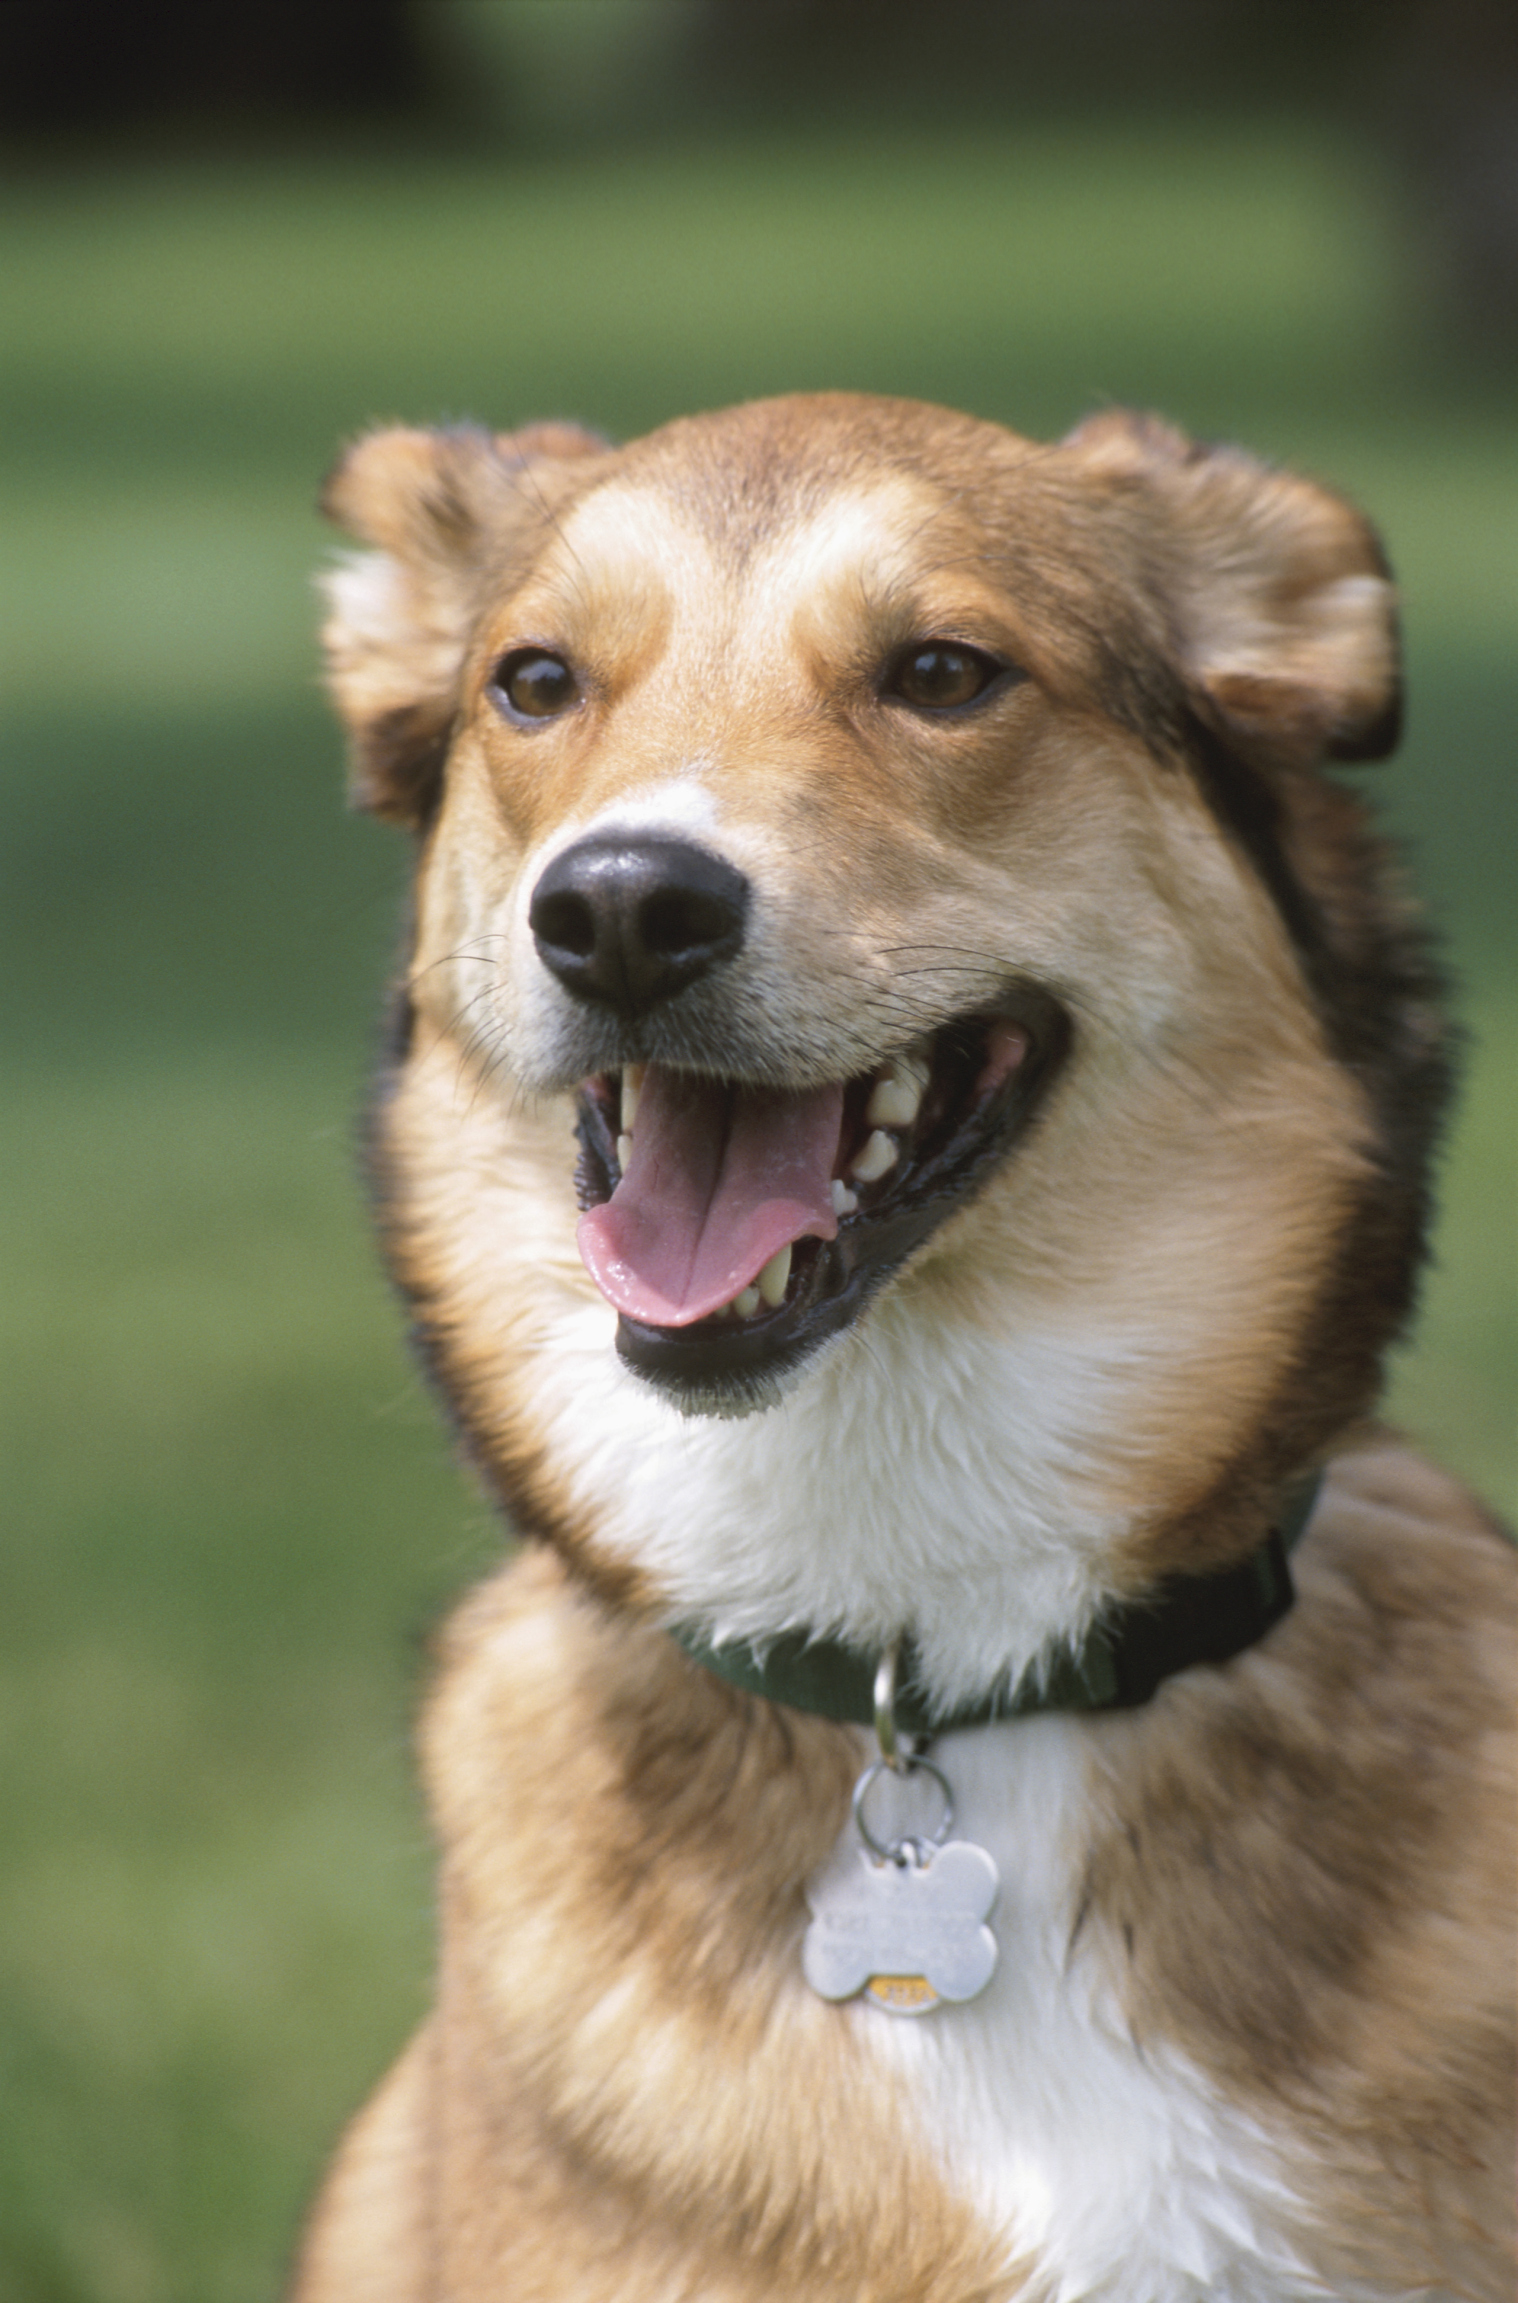
\includegraphics[width=\columnwidth]{fig/dog3-collar.jpg}
    \caption{alpha}
  \end{subfigure}
  \hfill
  \begin{subfigure}{0.2\columnwidth}
    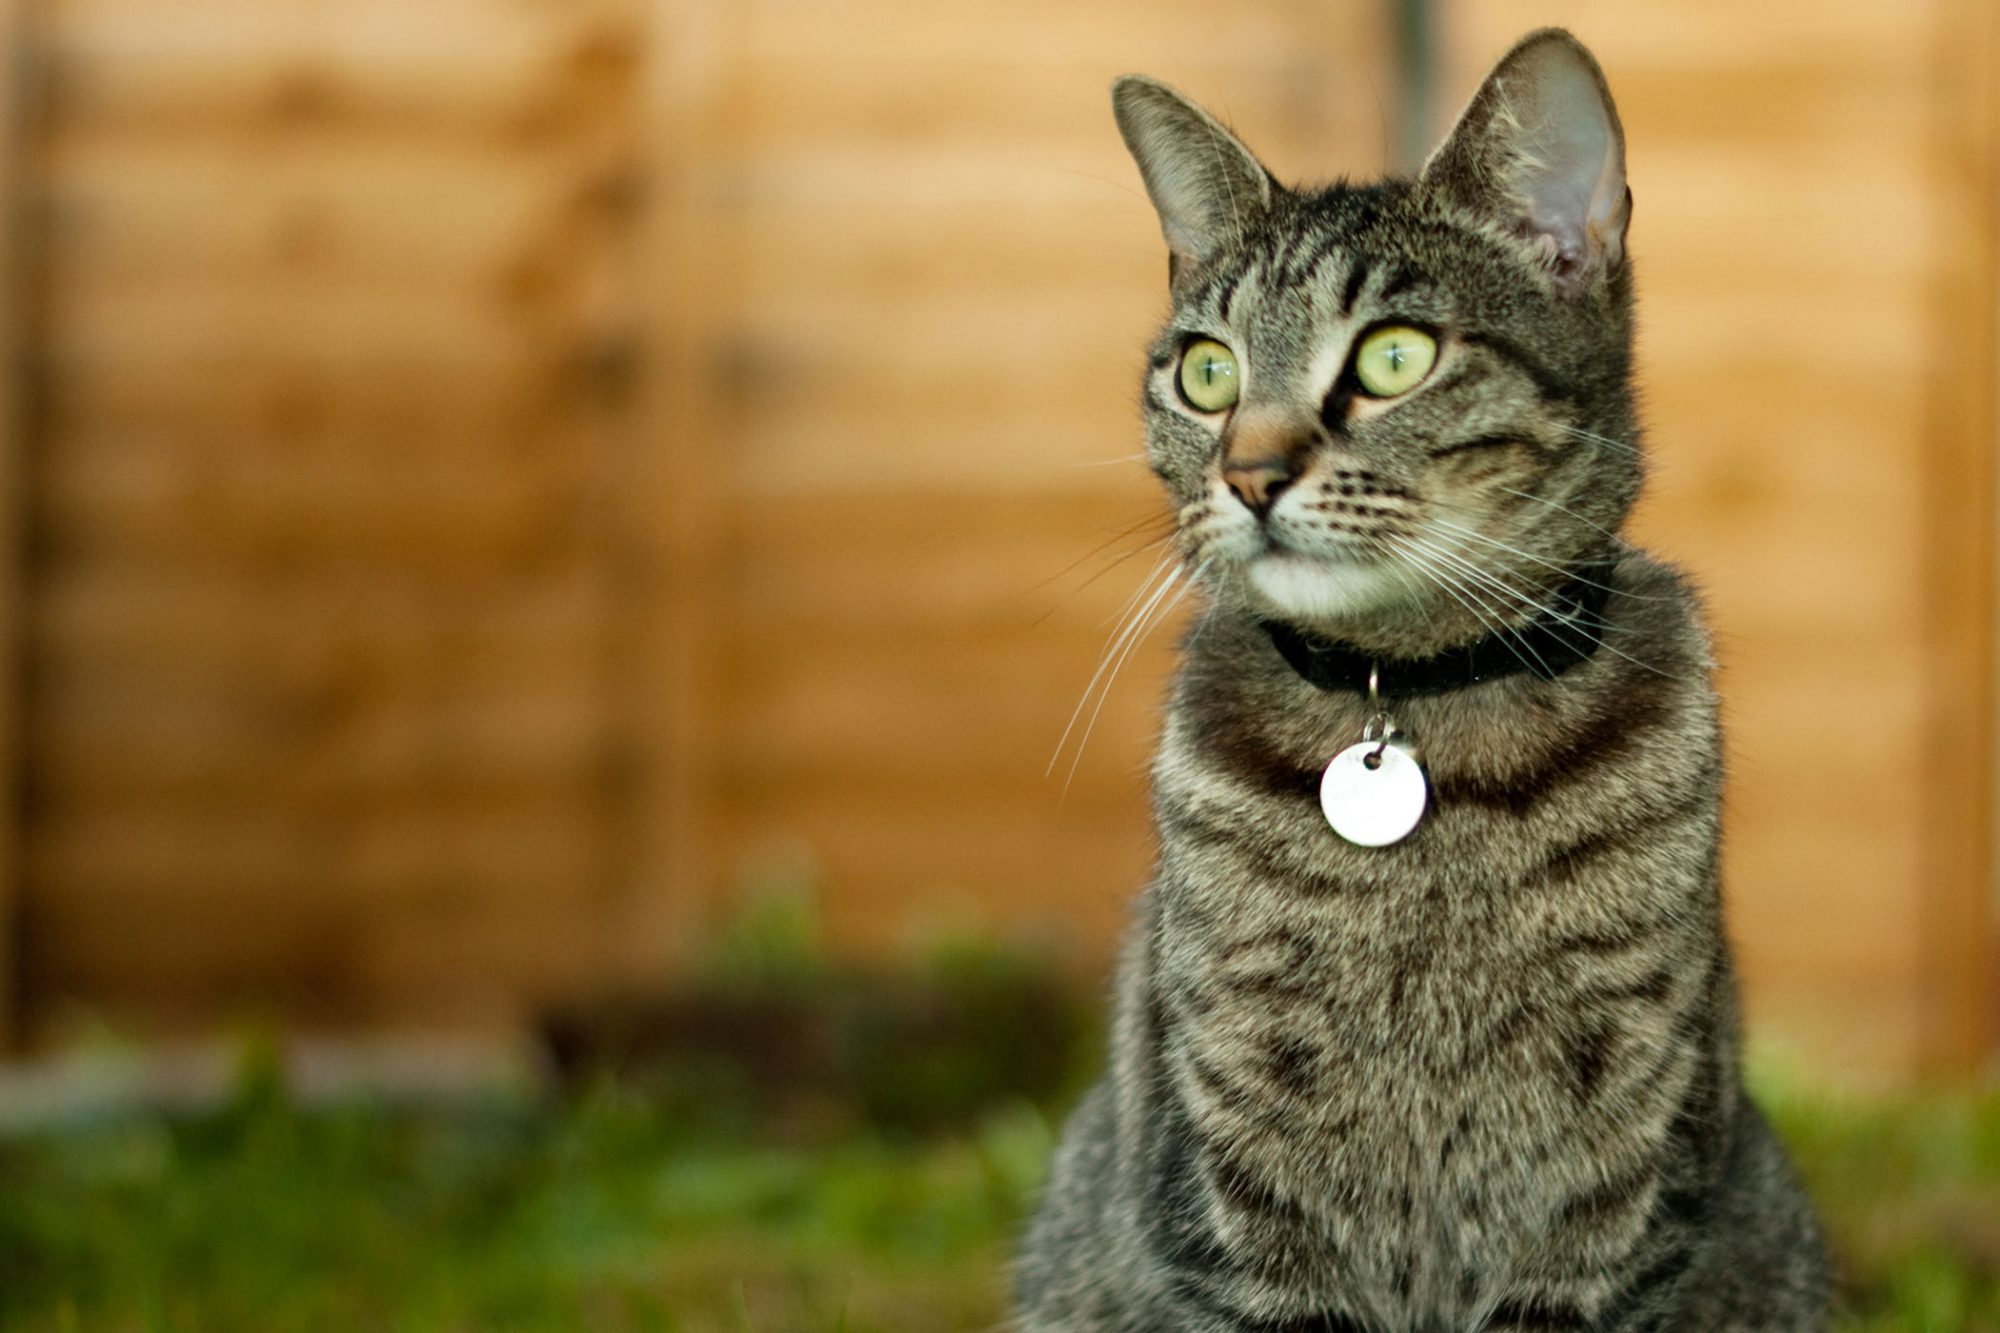
\includegraphics[width=\columnwidth]{fig/cat-collar.jpeg}
    \caption{alpha}
  \end{subfigure}
  \hfill
  \begin{subfigure}{0.2\columnwidth}
    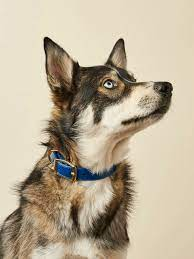
\includegraphics[width=\columnwidth]{fig/dog2-collar.jpeg}
    \caption{alpha}
  \end{subfigure}
  \hfill
  \begin{subfigure}{0.2\columnwidth}
    
\includegraphics[width=\columnwidth]{fig/cat2-collar.jpeg}
    \caption{alpha}
  \end{subfigure}
  \caption{Generalizing examples of alpha}
\end{figure}
}

\begin{frame}
  \begin{question}
    \begin{enumerate}
      \item What does \enquote{alpha} mean?
      \item How certain are you?
    \end{enumerate}
  \end{question}
\end{frame}

\mode<all>{\begin{frame}
  \begin{figure}
    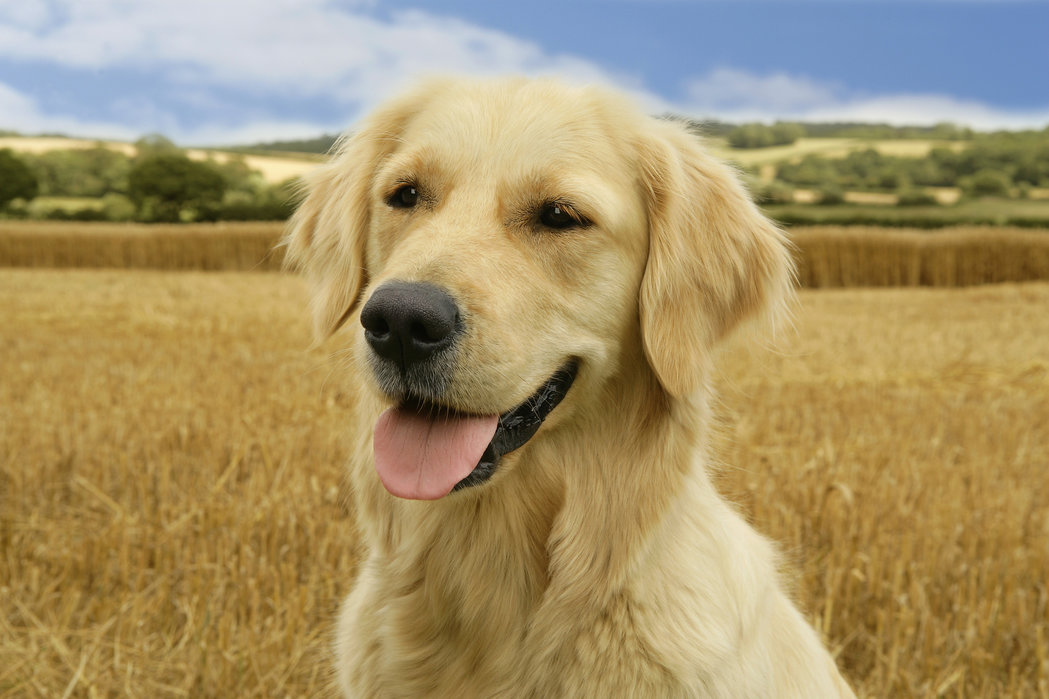
\includegraphics[height=0.8\textheight]{fig/golden-retriever.jpg}
    \caption{Example of \emph{not} alpha}
  \end{figure}
\end{frame}

\begin{frame}
  \begin{figure}
    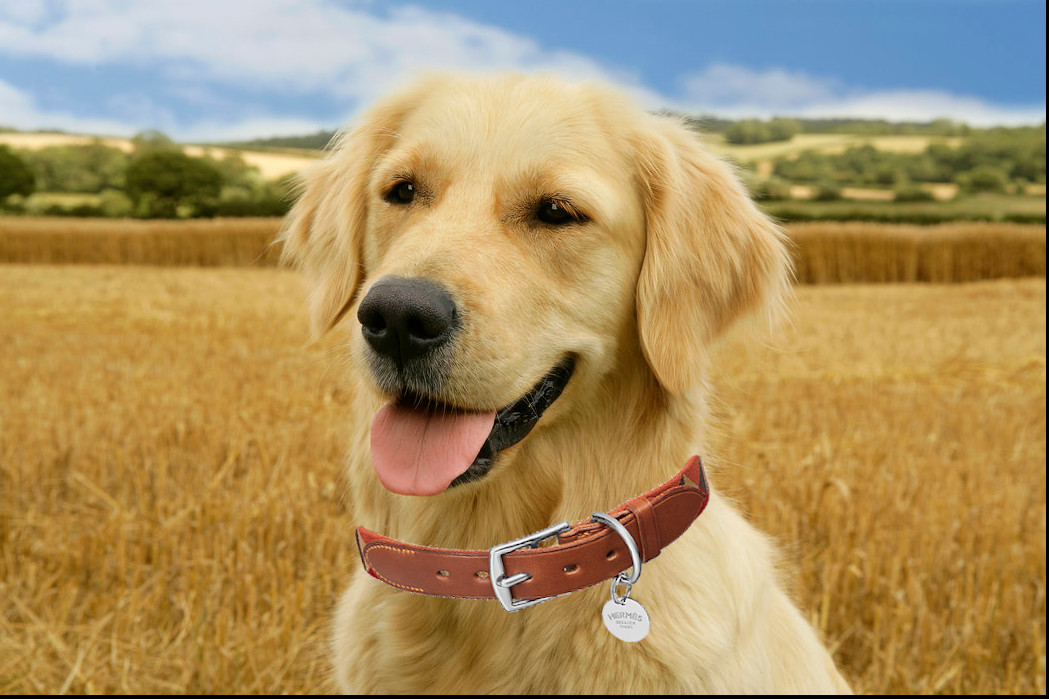
\includegraphics[height=0.8\textheight]{fig/golden-retriever-collar.jpg}
    \caption{Example of alpha}
  \end{figure}
\end{frame}

}
\mode<all>{\begin{figure}
  \begin{subfigure}{0.2\columnwidth}
    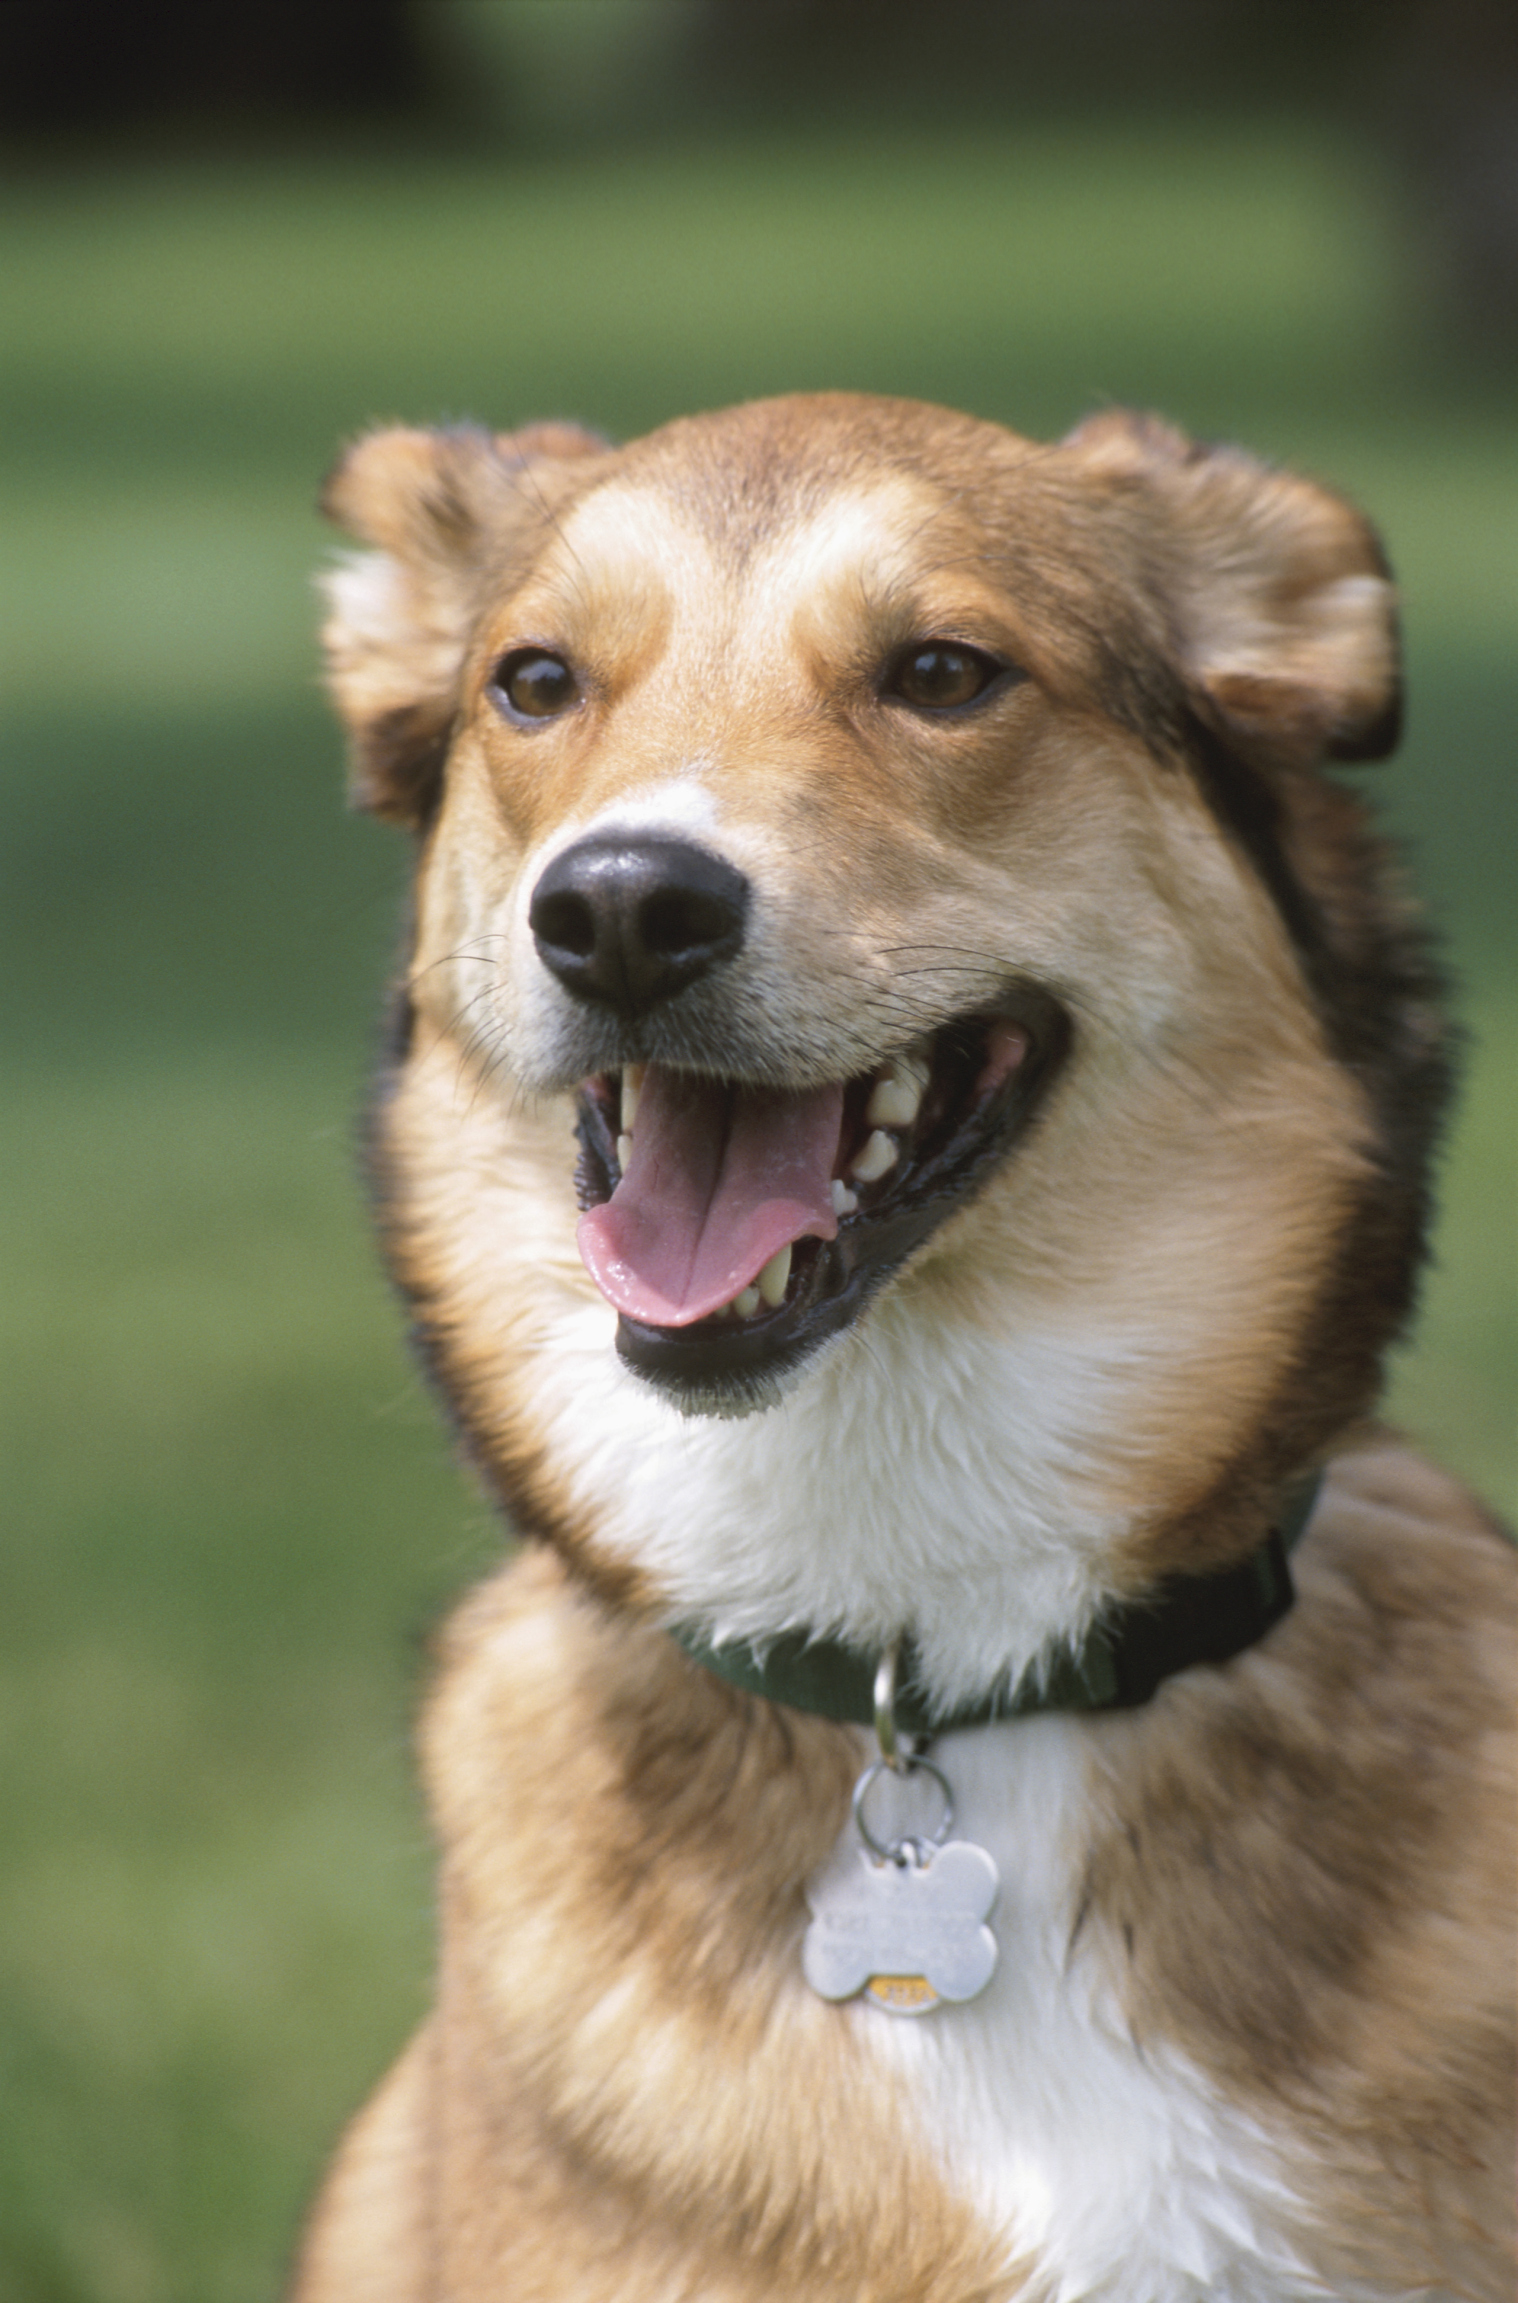
\includegraphics[width=\columnwidth]{fig/dog3-collar.jpg}
    \caption{alpha}
  \end{subfigure}
  \hfill
  \begin{subfigure}{0.2\columnwidth}
    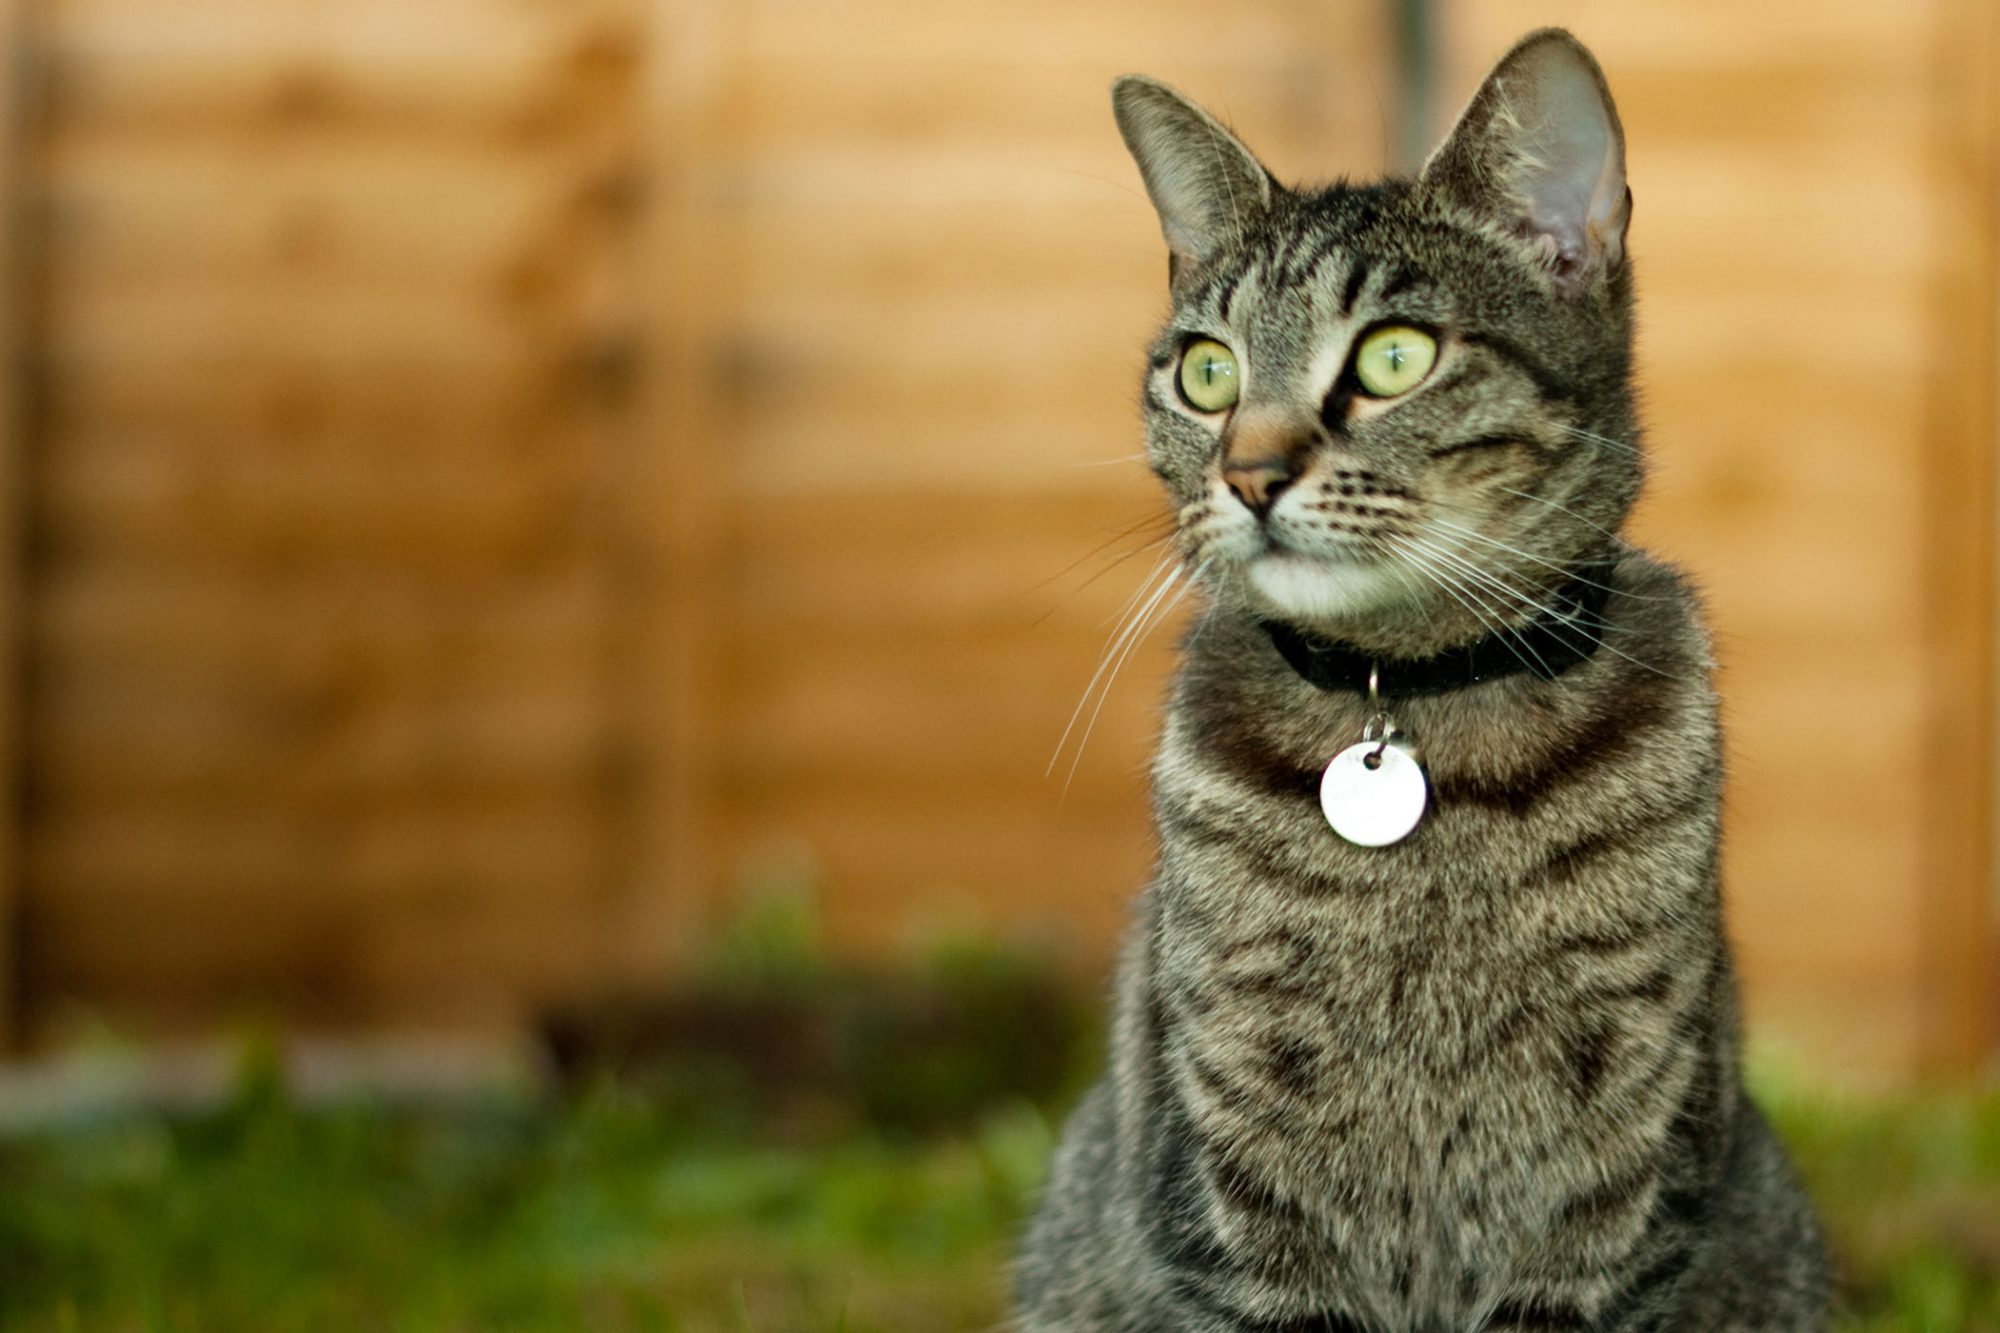
\includegraphics[width=\columnwidth]{fig/cat-collar.jpeg}
    \caption{alpha}
  \end{subfigure}
  \hfill
  \begin{subfigure}{0.2\columnwidth}
    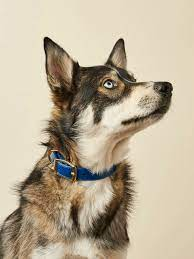
\includegraphics[width=\columnwidth]{fig/dog2-collar.jpeg}
    \caption{alpha}
  \end{subfigure}
  \hfill
  \begin{subfigure}{0.2\columnwidth}
    
\includegraphics[width=\columnwidth]{fig/cat2-collar.jpeg}
    \caption{alpha}
  \end{subfigure}
  \caption{Generalizing examples of alpha}
\end{figure}
}

\begin{frame}
  \begin{question}[Again]
    \begin{enumerate}
      \item What does \enquote{alpha} mean?
      \item How certain are you?
    \end{enumerate}
  \end{question}
\end{frame}

\begin{frame}
  \begin{remark}
    \begin{itemize}
      \item Finally I gave you the \emph{contrast}.
      \item You already had the \emph{generalization}, but as \emph{induction}.
    \end{itemize}
  \end{remark}
\end{frame}

